% Section 3, the BESSER chain: \input by report_2.tex, so that editing it never conflicts with the rest.

In one sentence: the BESSER chain takes a description of the exams, turns it step by step into a quantum
circuit, runs that circuit on a simulator, and turns the answers back into a timetable that a person can read.
Every step reads a model and writes a model, and every model it writes is saved in
\texttt{besser/output/<instance>/}, so each step can be opened and checked on its own.
\Cref{fig:besser-chain} follows the smallest example, \texttt{tiny} (3 exams, 3 time slots, 9 qubits).

\begin{figure}
	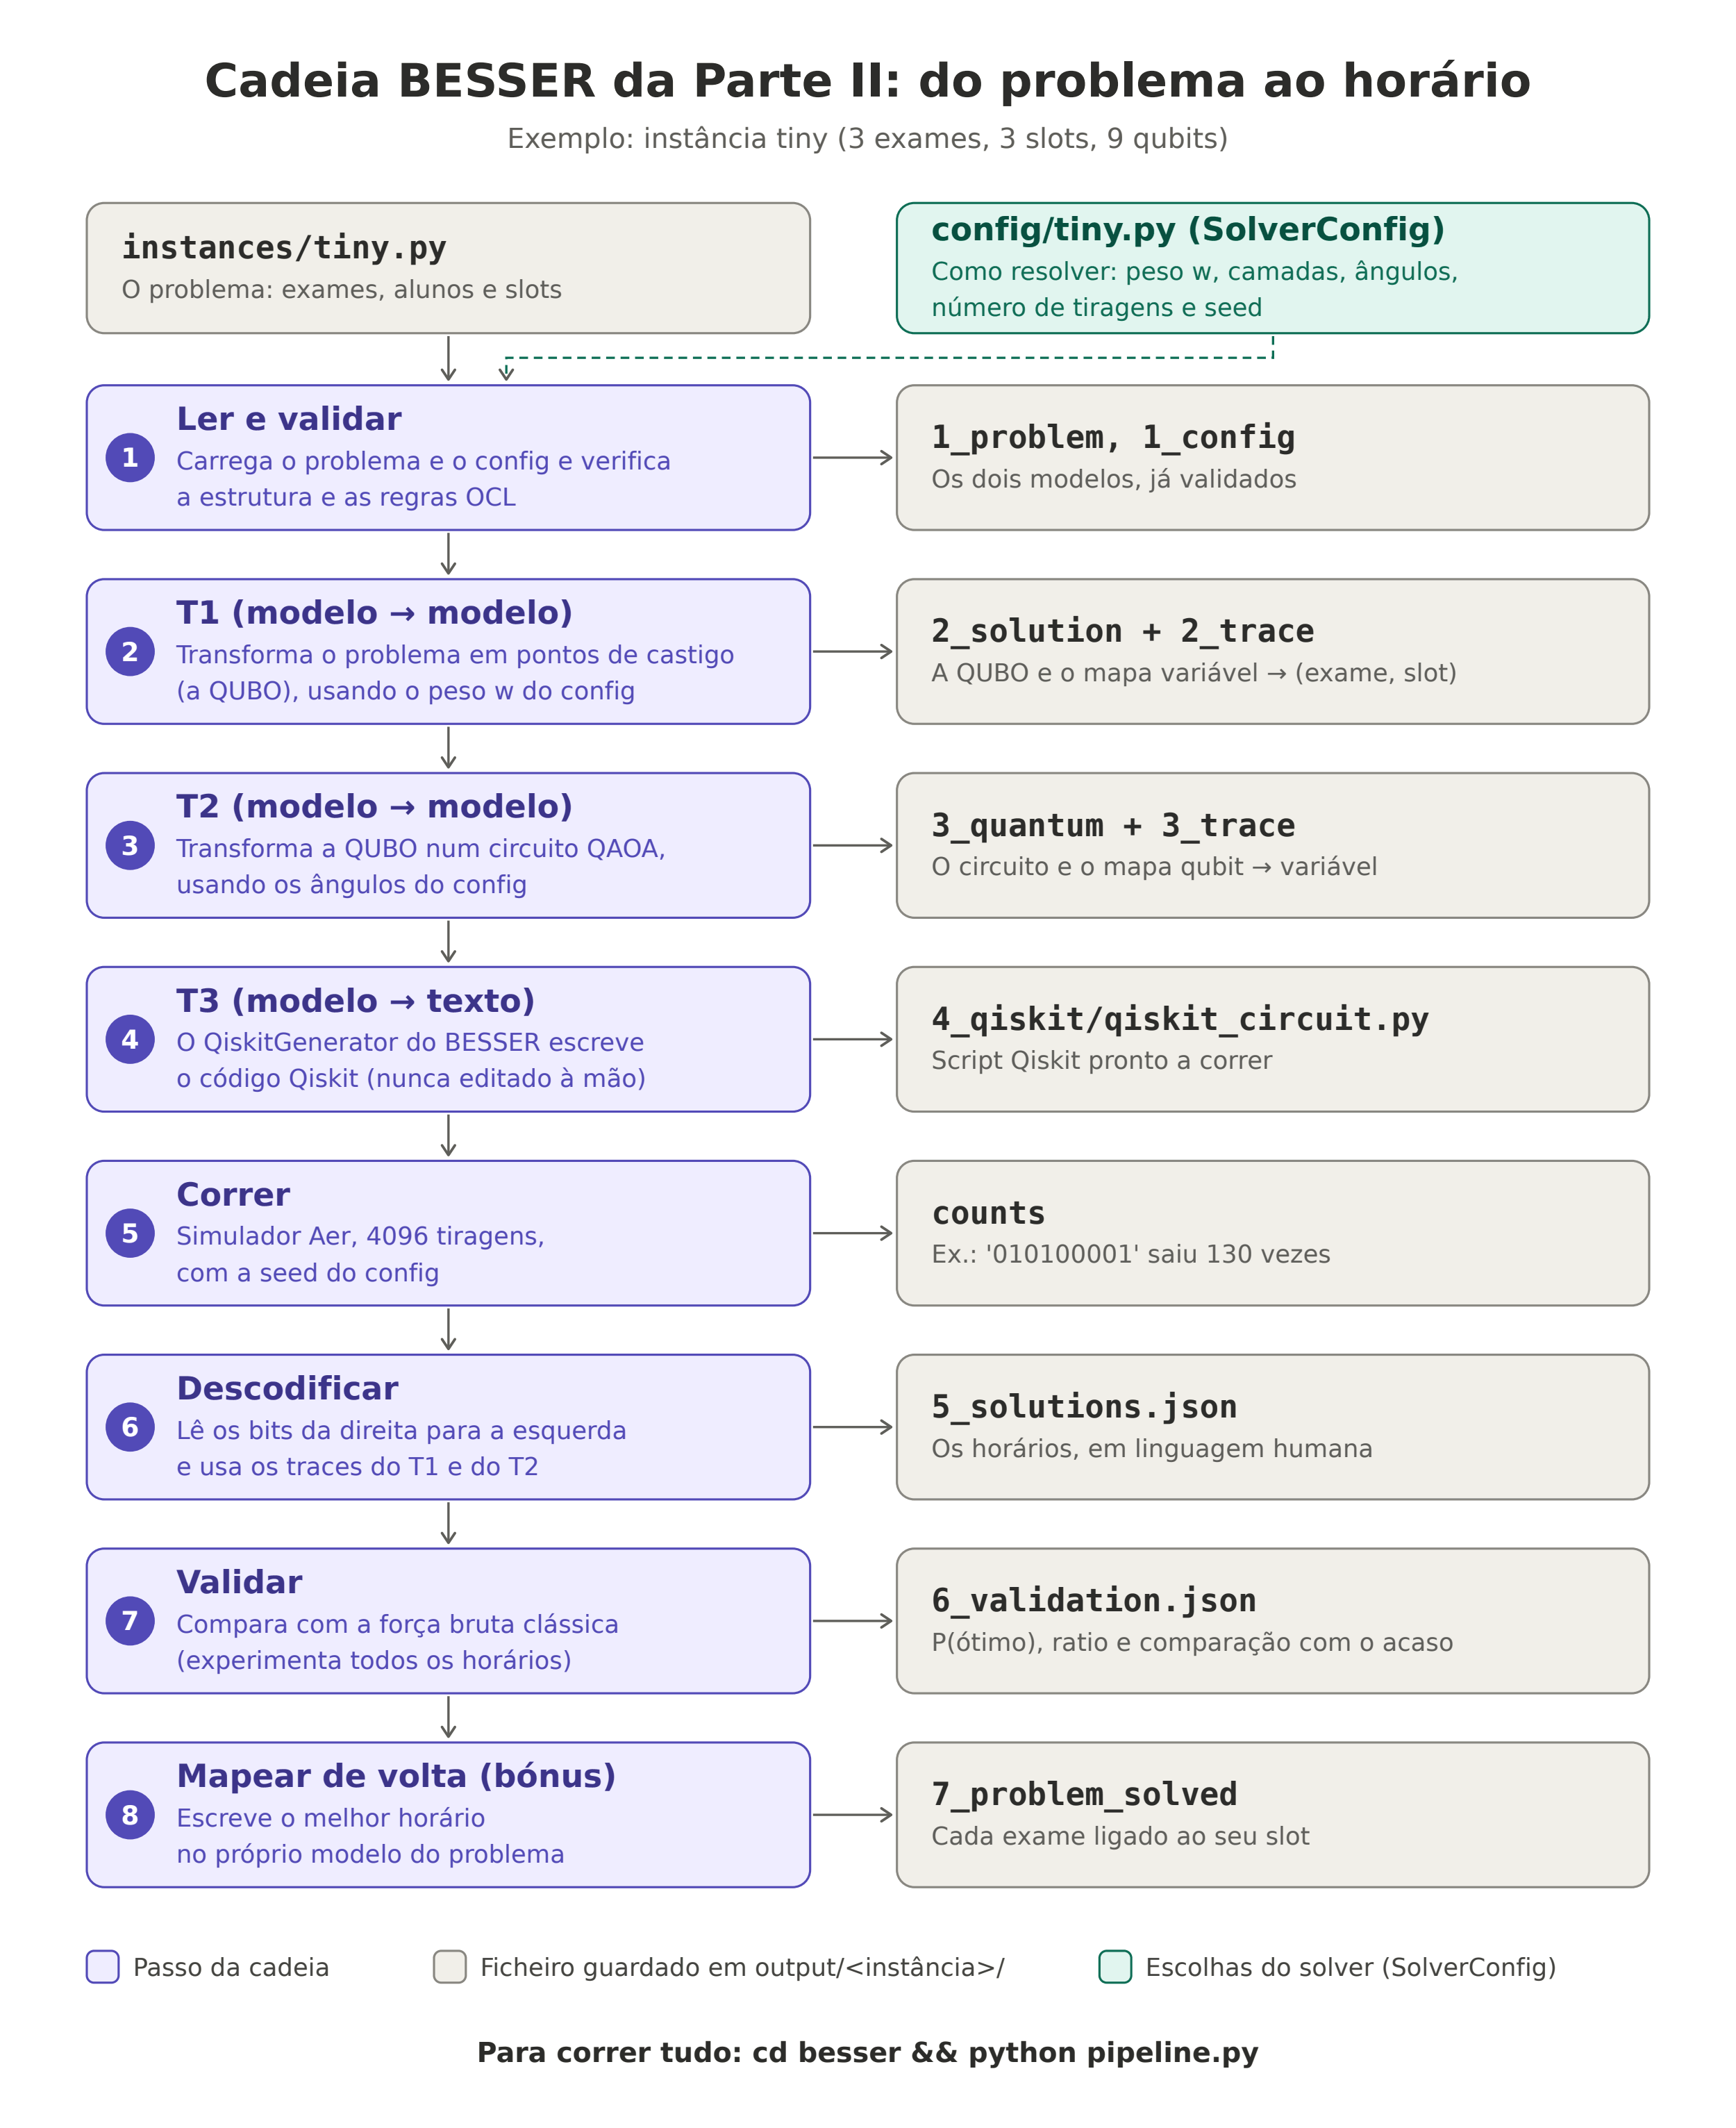
\includegraphics[width=\linewidth]{../imgs/cadeia_besser-1.png}
	\caption{The BESSER chain on the \texttt{tiny} instance: each step (left) and the model it saves (right).}
	\label{fig:besser-chain}
\end{figure}

\paragraph{Two inputs: the \emph{what} and the \emph{how}.}
Everything starts from two files written by a person. The first describes \emph{the problem}: the exams,
the students who sit them, and the time slots (\texttt{instances/tiny.py}, a model of Part~I's Problem
DSL). The second says \emph{how to solve it}: how much a conflict costs, how many layers the circuit has,
its angles, how many times to run it, and a seed so that every run gives the same result
(\texttt{config/tiny.py}, a model of our Solver Configuration metamodel). They are kept apart on purpose:
to solve the same problem in another way, only the configuration changes, never the code.

\begin{enumerate}
	\item \textbf{Read and check.} Both models are loaded and checked against the rules of their
	      metamodels, written in OCL: for example, an exam must have a name, and the number of circuit
	      layers must match the depth. If a rule fails, the chain stops here.
	      Saved: \texttt{1\_problem}, \texttt{1\_config}.
	\item \textbf{T1, model to model: from exams to penalty points.} The problem becomes a QUBO, a list of
	      penalty points. There is one yes/no variable for each pair (exam, slot), and a schedule earns
	      points for every rule it breaks: an exam with no slot or with two slots, or two exams that share a
	      student placed in the same slot \cite[§5.3]{Paper}. A schedule with zero points is a valid one.
	      Leaving an exam out always costs more than a conflict, so the solver cannot ``cheat'' by dropping
	      an exam \cite[§2.3]{Lucas}. Saved: \texttt{2\_solution}, and a trace from each variable to its
	      exam and slot.
	\item \textbf{T2, model to model: from penalty points to a quantum circuit.} The QUBO becomes a QAOA
	      circuit \cite{Farhi} in BESSER's own quantum metamodel: one qubit per variable, and layers that
	      push the qubits towards the schedules with fewer points. The angles of each layer come from the
	      configuration. Saved: \texttt{3\_quantum}, and a trace from each qubit to its variable.
	\item \textbf{T3, model to text: writing the code.} BESSER's \texttt{QiskitGenerator} writes the
	      circuit as a Qiskit script, \texttt{4\_qiskit/qiskit\_circuit.py}. The generated code is never
	      edited by hand: if something is wrong, the model or the transformation is fixed.
	\item \textbf{Run.} The script runs on the Qiskit Aer simulator \cite{Qiskit} 4096 times, with the
	      seed of the configuration. The result is a count of how often each string of bits came out.
	\item \textbf{Decode.} Each string of bits is read from right to left, as Qiskit writes it, and the two
	      traces turn every bit back into ``exam X in slot Y''. Saved: \texttt{5\_solutions.json}, the
	      schedules in plain words, with the rules each one breaks.
	\item \textbf{Validate.} A classical program tries every possible schedule and finds the best ones.
	      The chain then measures how often the circuit found a valid schedule and a best schedule, and
	      compares this with picking a string of bits at random. Saved: \texttt{6\_validation.json}.
	\item \textbf{Map back.} The best schedule found is written into the problem model itself, each exam
	      linked to its slot, and checked again against the OCL rules. Saved: \texttt{7\_problem\_solved}.
\end{enumerate}

The whole chain runs with one command, \texttt{cd besser \&\& python pipeline.py}, in about two seconds
for the five instances.
